% !TEX root = dynamicslearning.tex

\section{Numerical experiments}\label{sec:num}
In order to convince the reader of the usefulness of Theorem \ref{thm}, we report below in Figure \ref{firstnum} one (of several we did) preliminary numerical experiment  indicating the successful recovery by an adaptive algorithm based on \eqref{fdproxy} of a potential function $a$ in a first order model of the type \eqref{fdgradientflow}. More specifically, we performed successive applications of  \eqref{fdproxy} based on an adaptive refinement of a mesh on the positive real line, defining approximating spaces $V$ of continuous piecewise linear functions. The adaptation is lead by a posteriori error estimator based on local comparison of two successive iterations.


\begin{figure}[h]
\begin{center}
 \includegraphics[width=0.3\textwidth]{Figure1}
\includegraphics[width=0.3\textwidth]{Figure3}
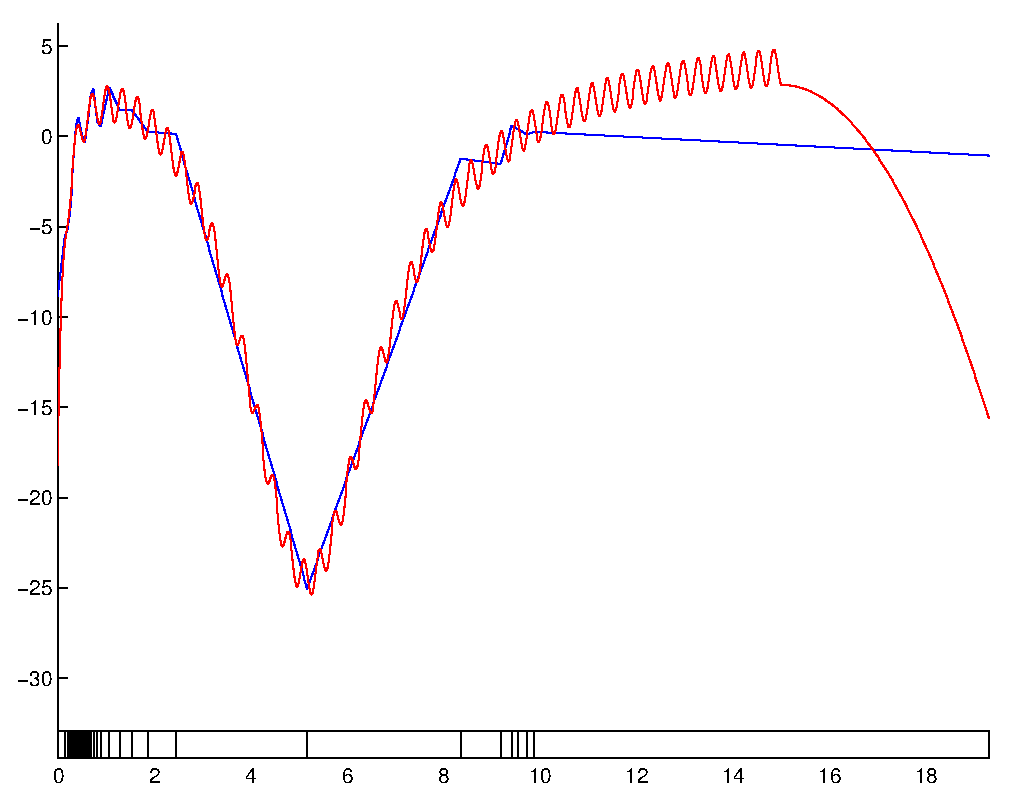
\includegraphics[width=0.3\textwidth]{Figure5}
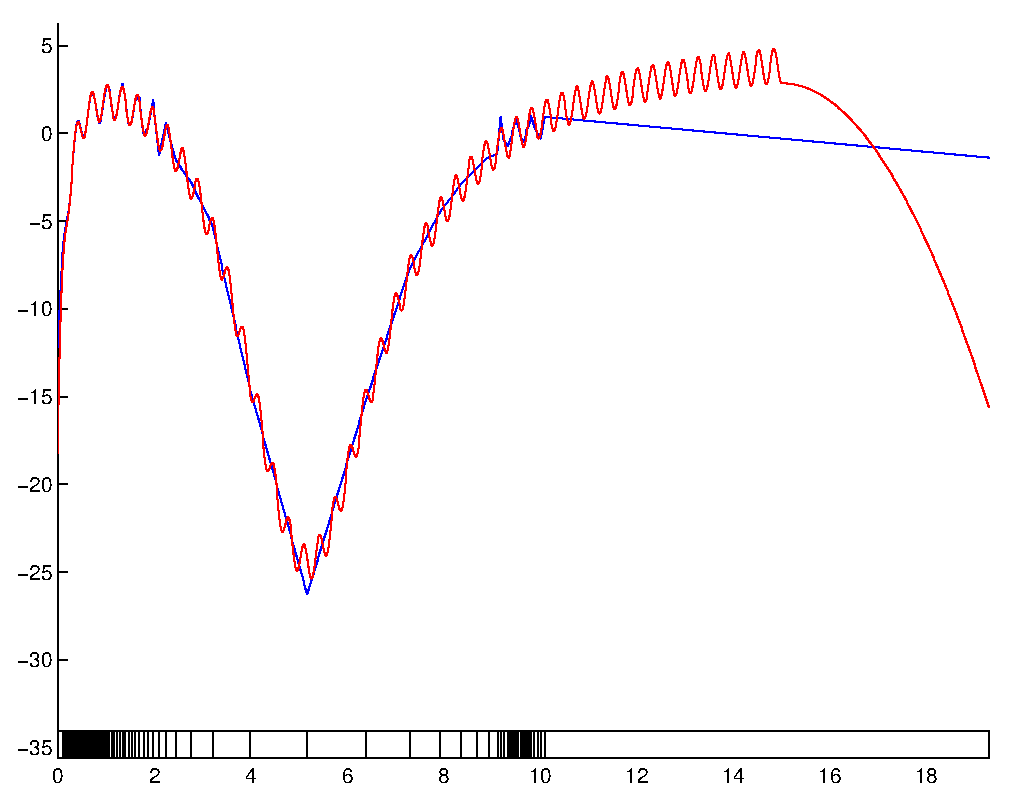
\includegraphics[width=0.3\textwidth]{Figure7}
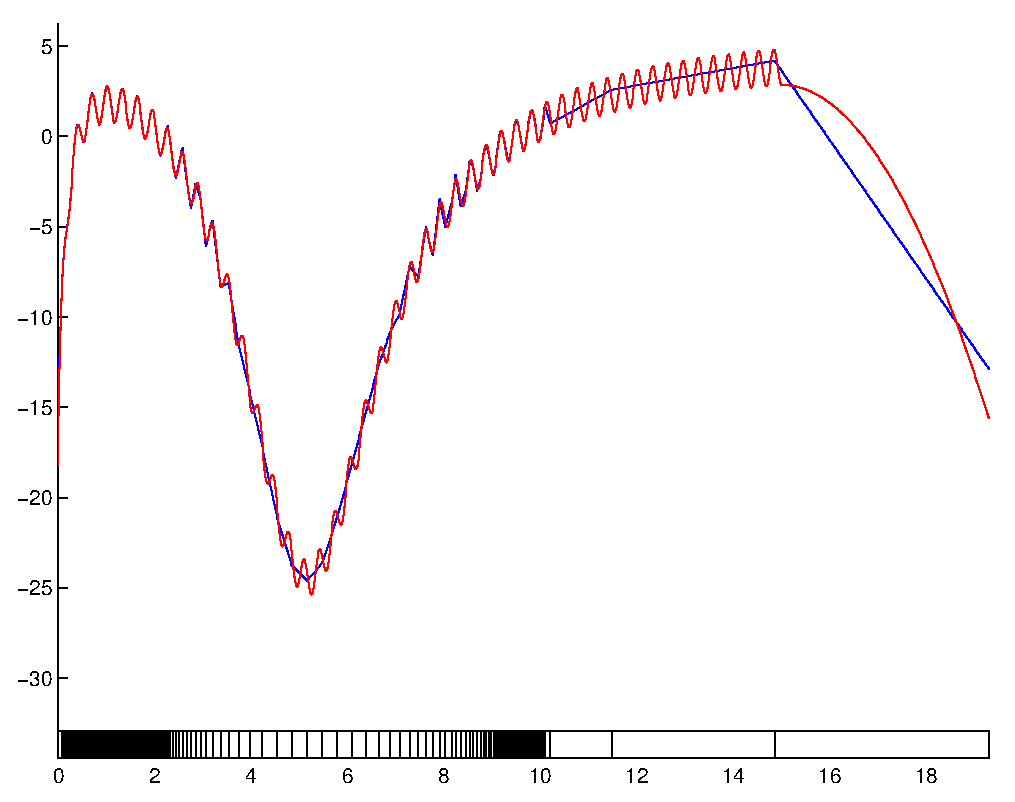
\includegraphics[width=0.3\textwidth]{Figure9}
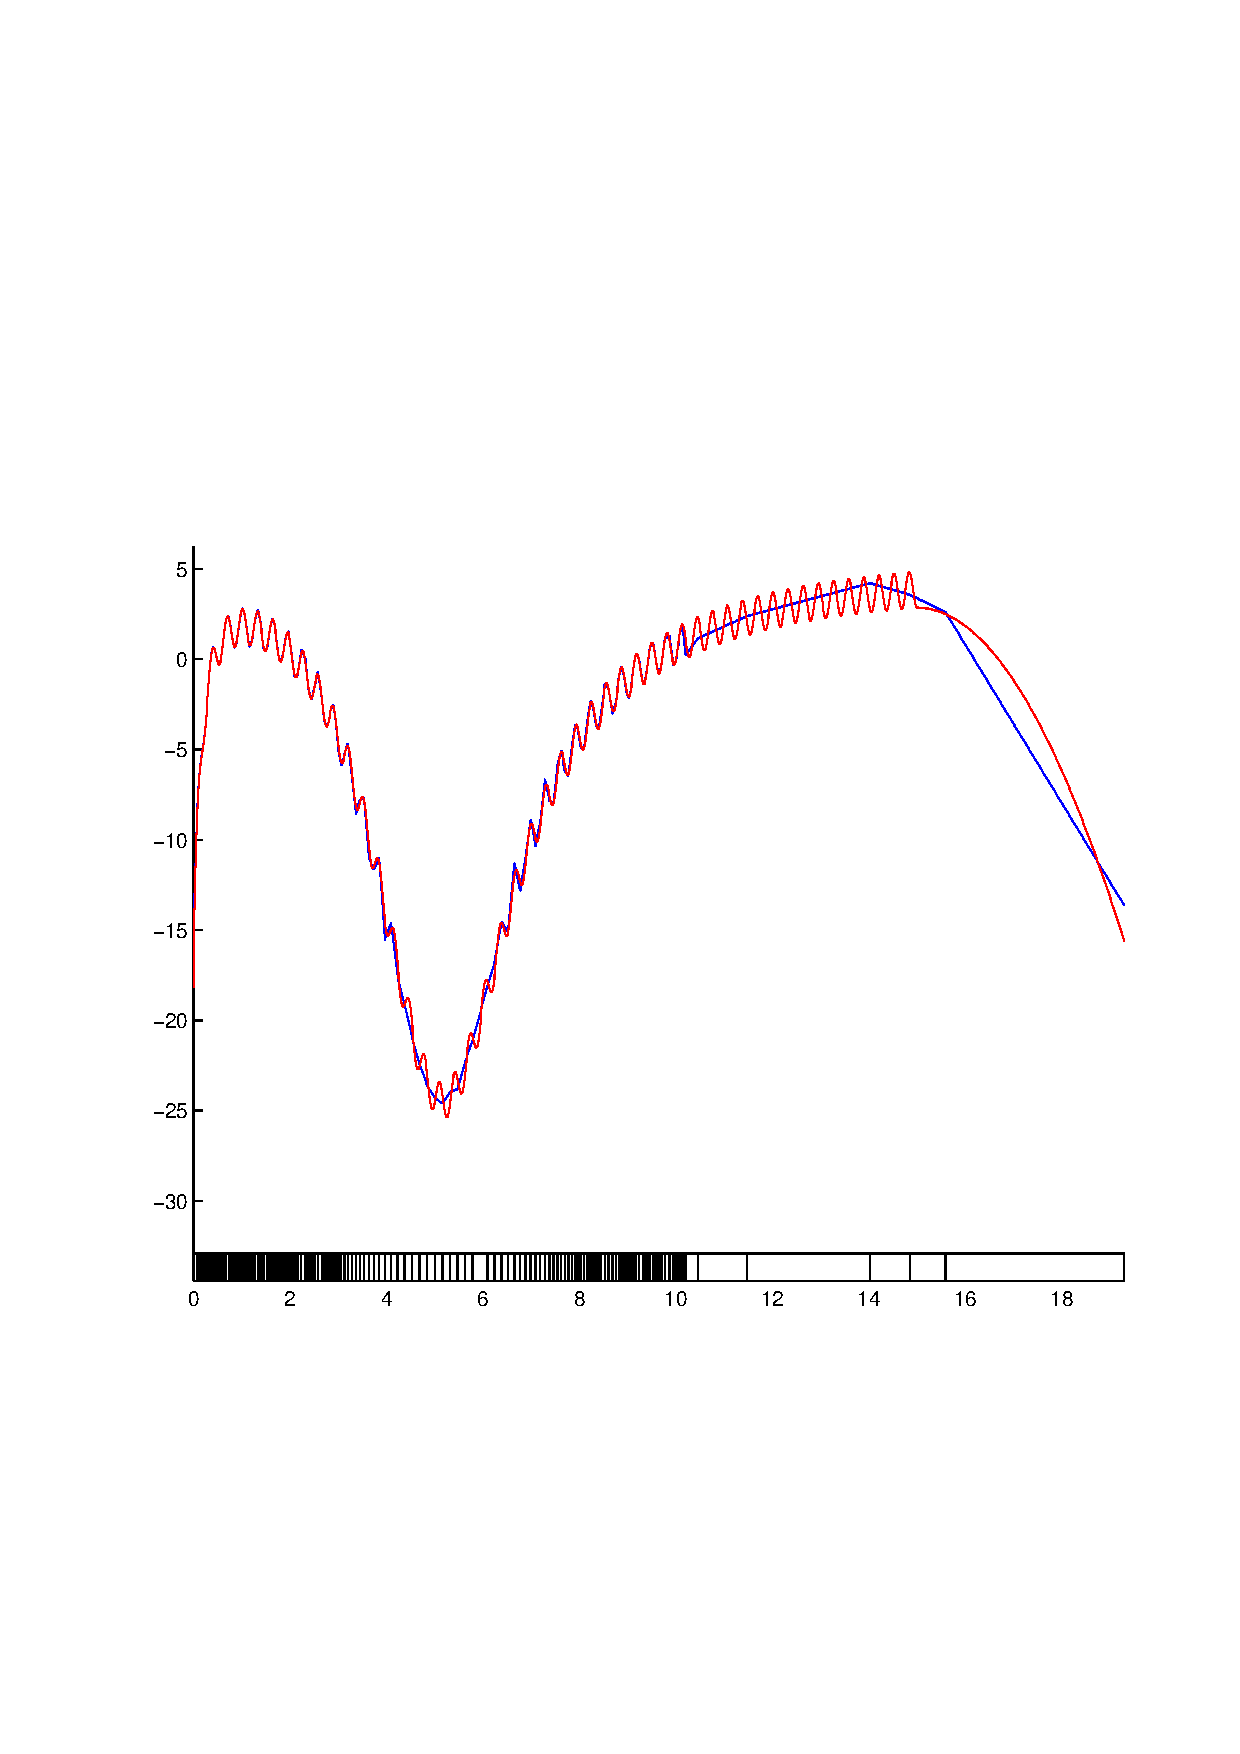
\includegraphics[width=0.3\textwidth]{Figure11} 
\end{center}
\caption{First preliminary numerical experiments indicating the successful recovery by an adaptive algorithm based on \eqref{fdproxy} of a potential function $a$ in a first order model of the type \eqref{fdgradientflow}. The potential $a$ to be recovered is displayed in red color and it's the strongly oscillating function. The blue function is the piecewise linear approximant computed at each successive iteration after adaptation of the underlying mesh, scketched on the bottom of the figures.}\label{firstnum}
\end{figure}

Despite the highly oscillatory nature of the parameter function $a$, the algorithm performs an excellent approximation, providing also a sort of "numerical homogenization" in those locations of the positive real line, where not enough data are provided by the evolution.